\subsubsection{Trabajos previos}
    En esta sección documenta los resultados obtenidos de las investigaciones propuestas como objetivo en este trabajo.
    Se ha consultado documentación y trabajos relacionados dentro del ámbito académico que respondan a la adecuación de Go como lenguaje para el desarrollo de sistemas como el realizado.
    Así como el protocolo de comunicación.
    \paragraph{Estudio justificativo del uso de Golang}
    En este apartado se responde al objetivo de analizar Go como lenguaje de programación enfocado a soluciones como la planteada.
    Para ello se ha realizado una investigación consultado trabajos relacionados para analizar las conclusiones.
    

\textbf{Golang}


Uno de los puntos centrales de este trabajo es exponer el estado del arte en el uso de Golang para el entorno industrial. En dicho estudio se ha consultado distintos papers y publicaciones para extraer primeras conclusiones:

Uno de los puntos más importantes para el desarrollo de software industrial es los recursos consumidos una de las primeras conclusines extraidas de la eficiencia del uso de golang interaccionando con mysql, una de las combinaciones más comerciales concluye que: "... combination of Go and MySQL is superior regarding CPU utilization and memory usage, while Node.js and MySQL combination is superior regarding response time~\cite{Effendy20211955}".

Un estudio más centrado en el uso de recursos ante problemas de algorítmia con altos requerimientos, en particular la implementacion de un árbol de decisiones. ~\cite{Dymora20201} Donde encontramos un punto importante: golang vuelve a no dar ventajas, pero tampoco inconvenientes en materia de tiempos de ejecucion. pero si que pierde en uso de cpu claramente y empata en materia de uso de memoria para mas de 500K registros en este problema en particular. Aunque se admite que la optimización de dicho mecanismo para este problema. lo cual es posible. "Thus, the Go language garbage collector
supports programmers by automatically releasing their programs’ memory when it is no longer needed.
However, tracking and cleaning the memory requires additional resources such as CPU time. The effect
of this can be seen in Figure 5. Of course, the scope of optimizing"~\cite{Dymora20201}

lo que si nos permite extraer es una conclusion y es que para usos intensivos golang es una opción viable pero no da ventaja en este aspecto.

Esto se debe al mecanismo que le da una ventaja tan notoria en el uso menos intensivo: el garbage collector que le requiere un uso adicional de memoria y cpu para ejecuciones con un gran número de registros. Concluye este estudio diciendo: ". Go can be an
attractive alternative in the area of DevOps tools. It is attractive to build something small–medium
that works natively without using a lot of RAM and which runs fast with many things needed for
this task in the language itself"~\cite{Dymora20201}

\begin{figure}[H]
	\centering
	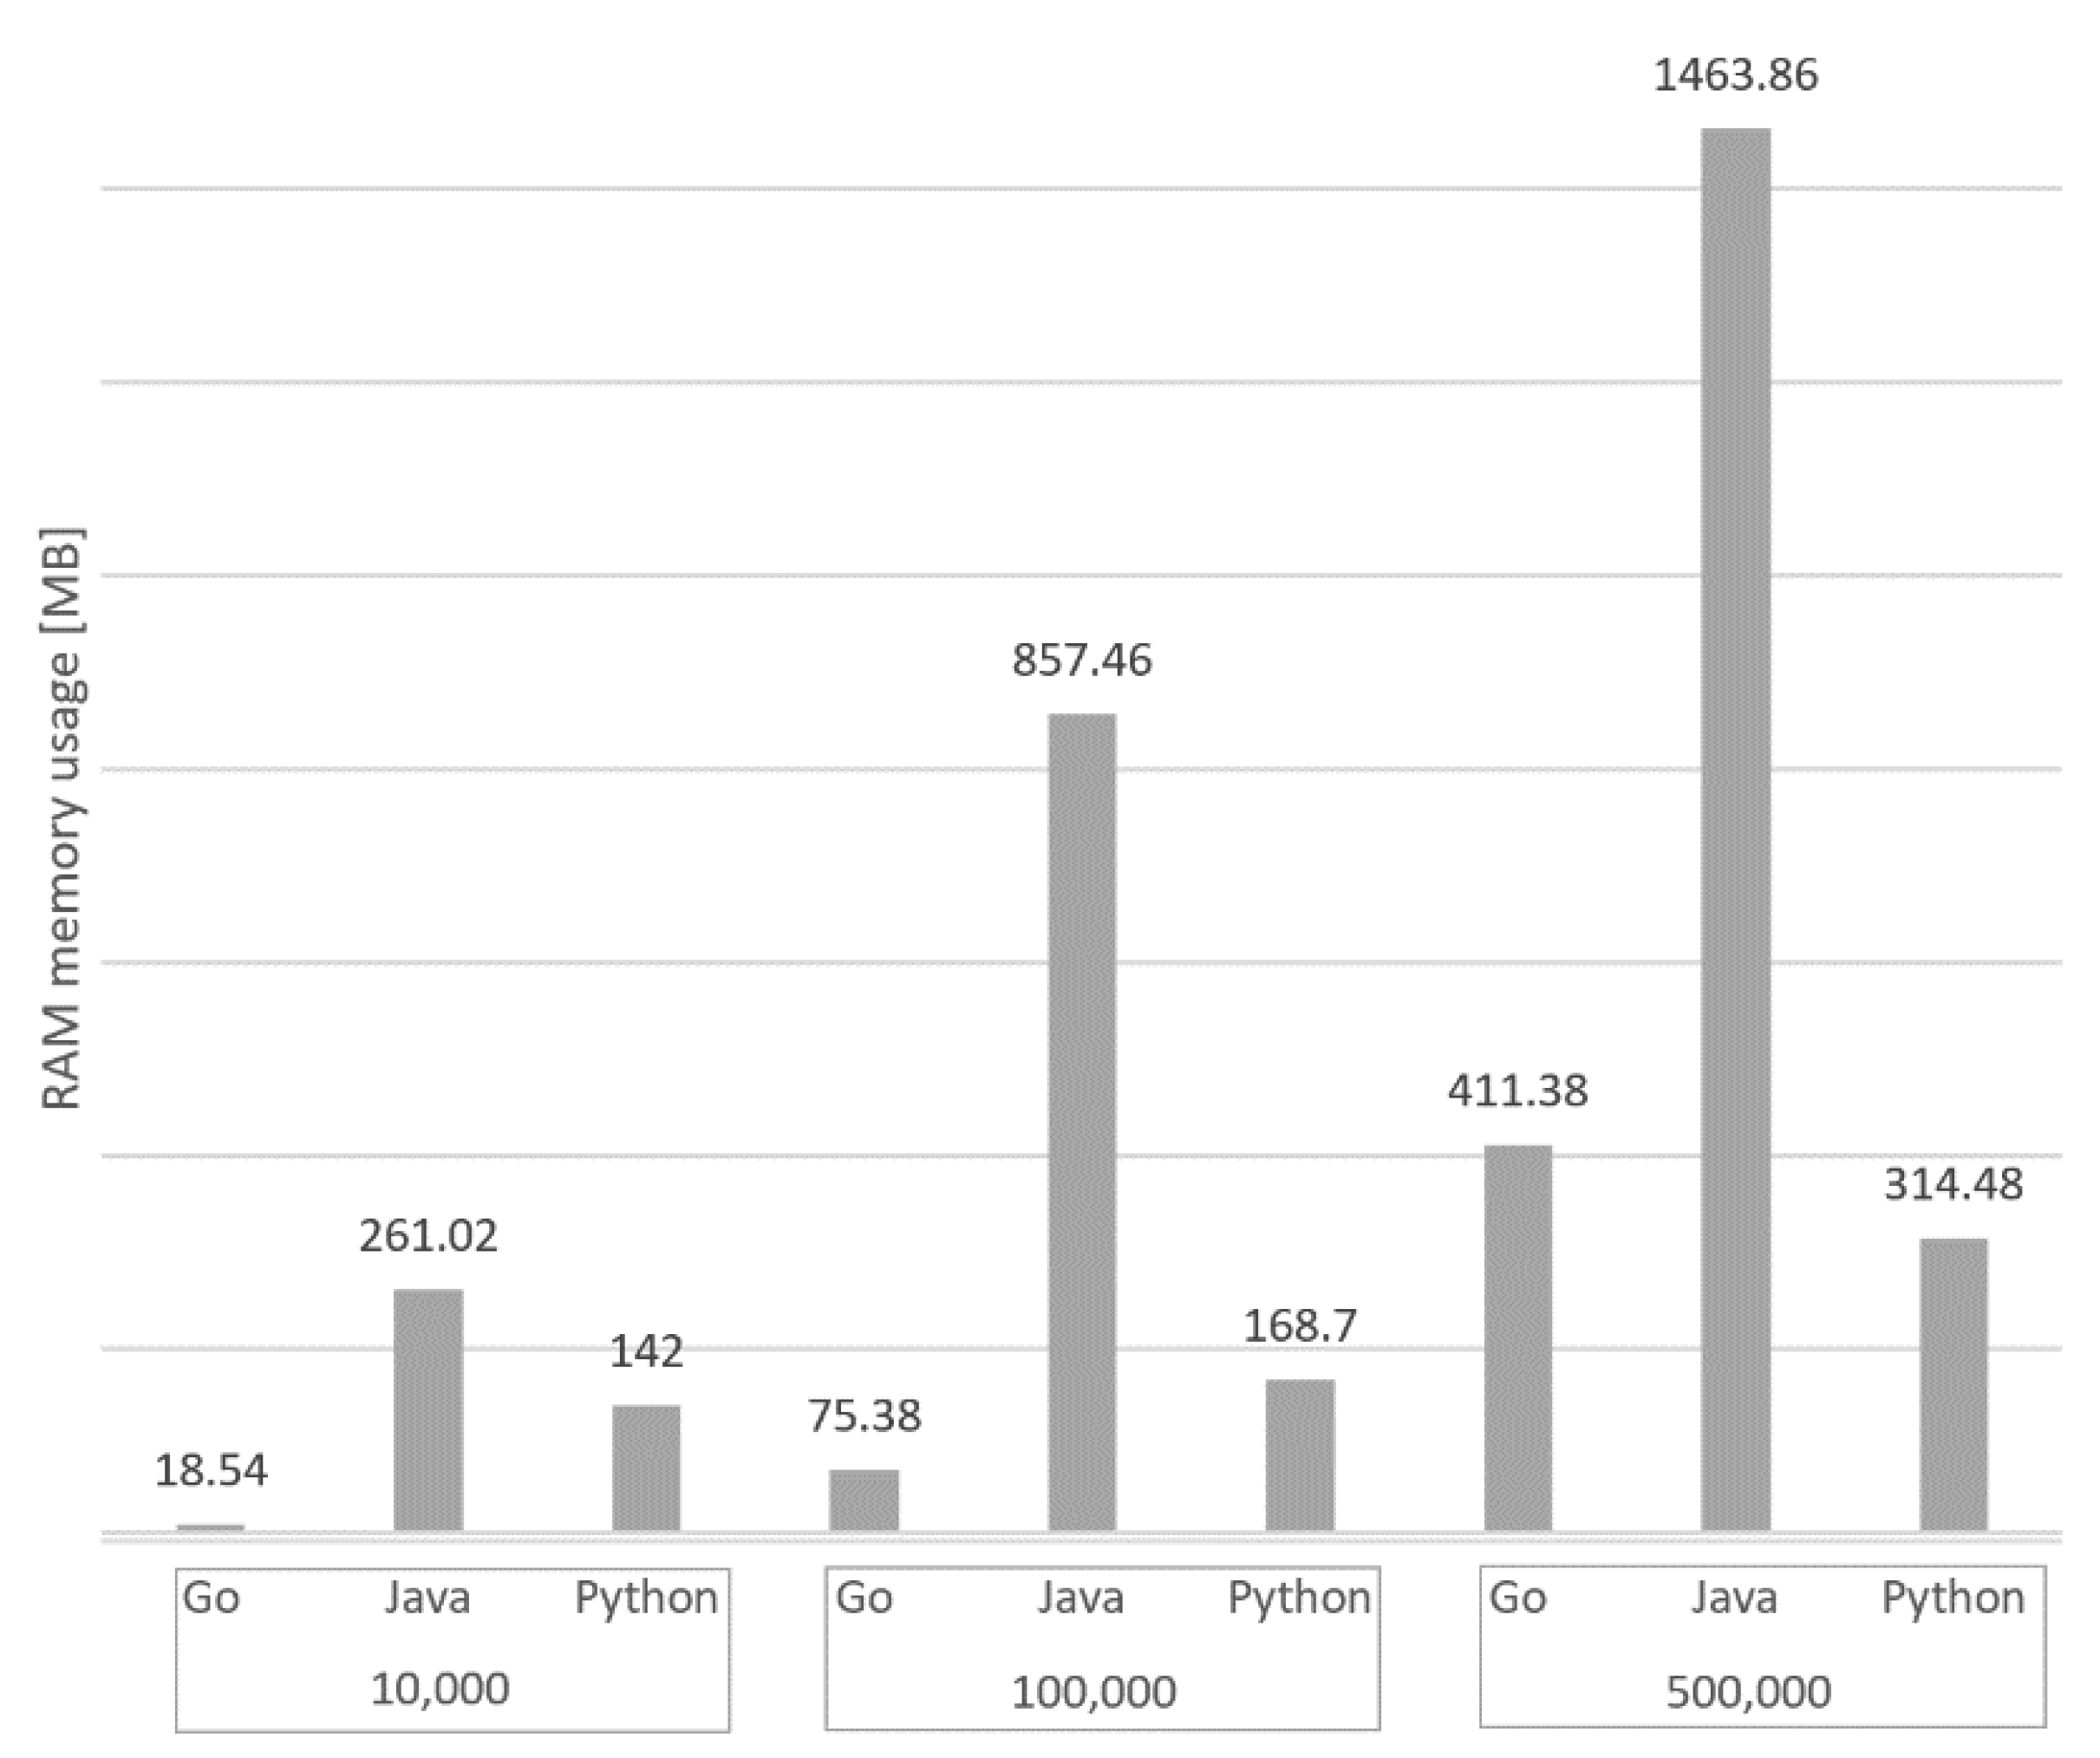
\includegraphics[height=0.3\textheight]{./part/Proyecto_ejecutivo/memoria_constructiva/golang/img/memory_usage}
	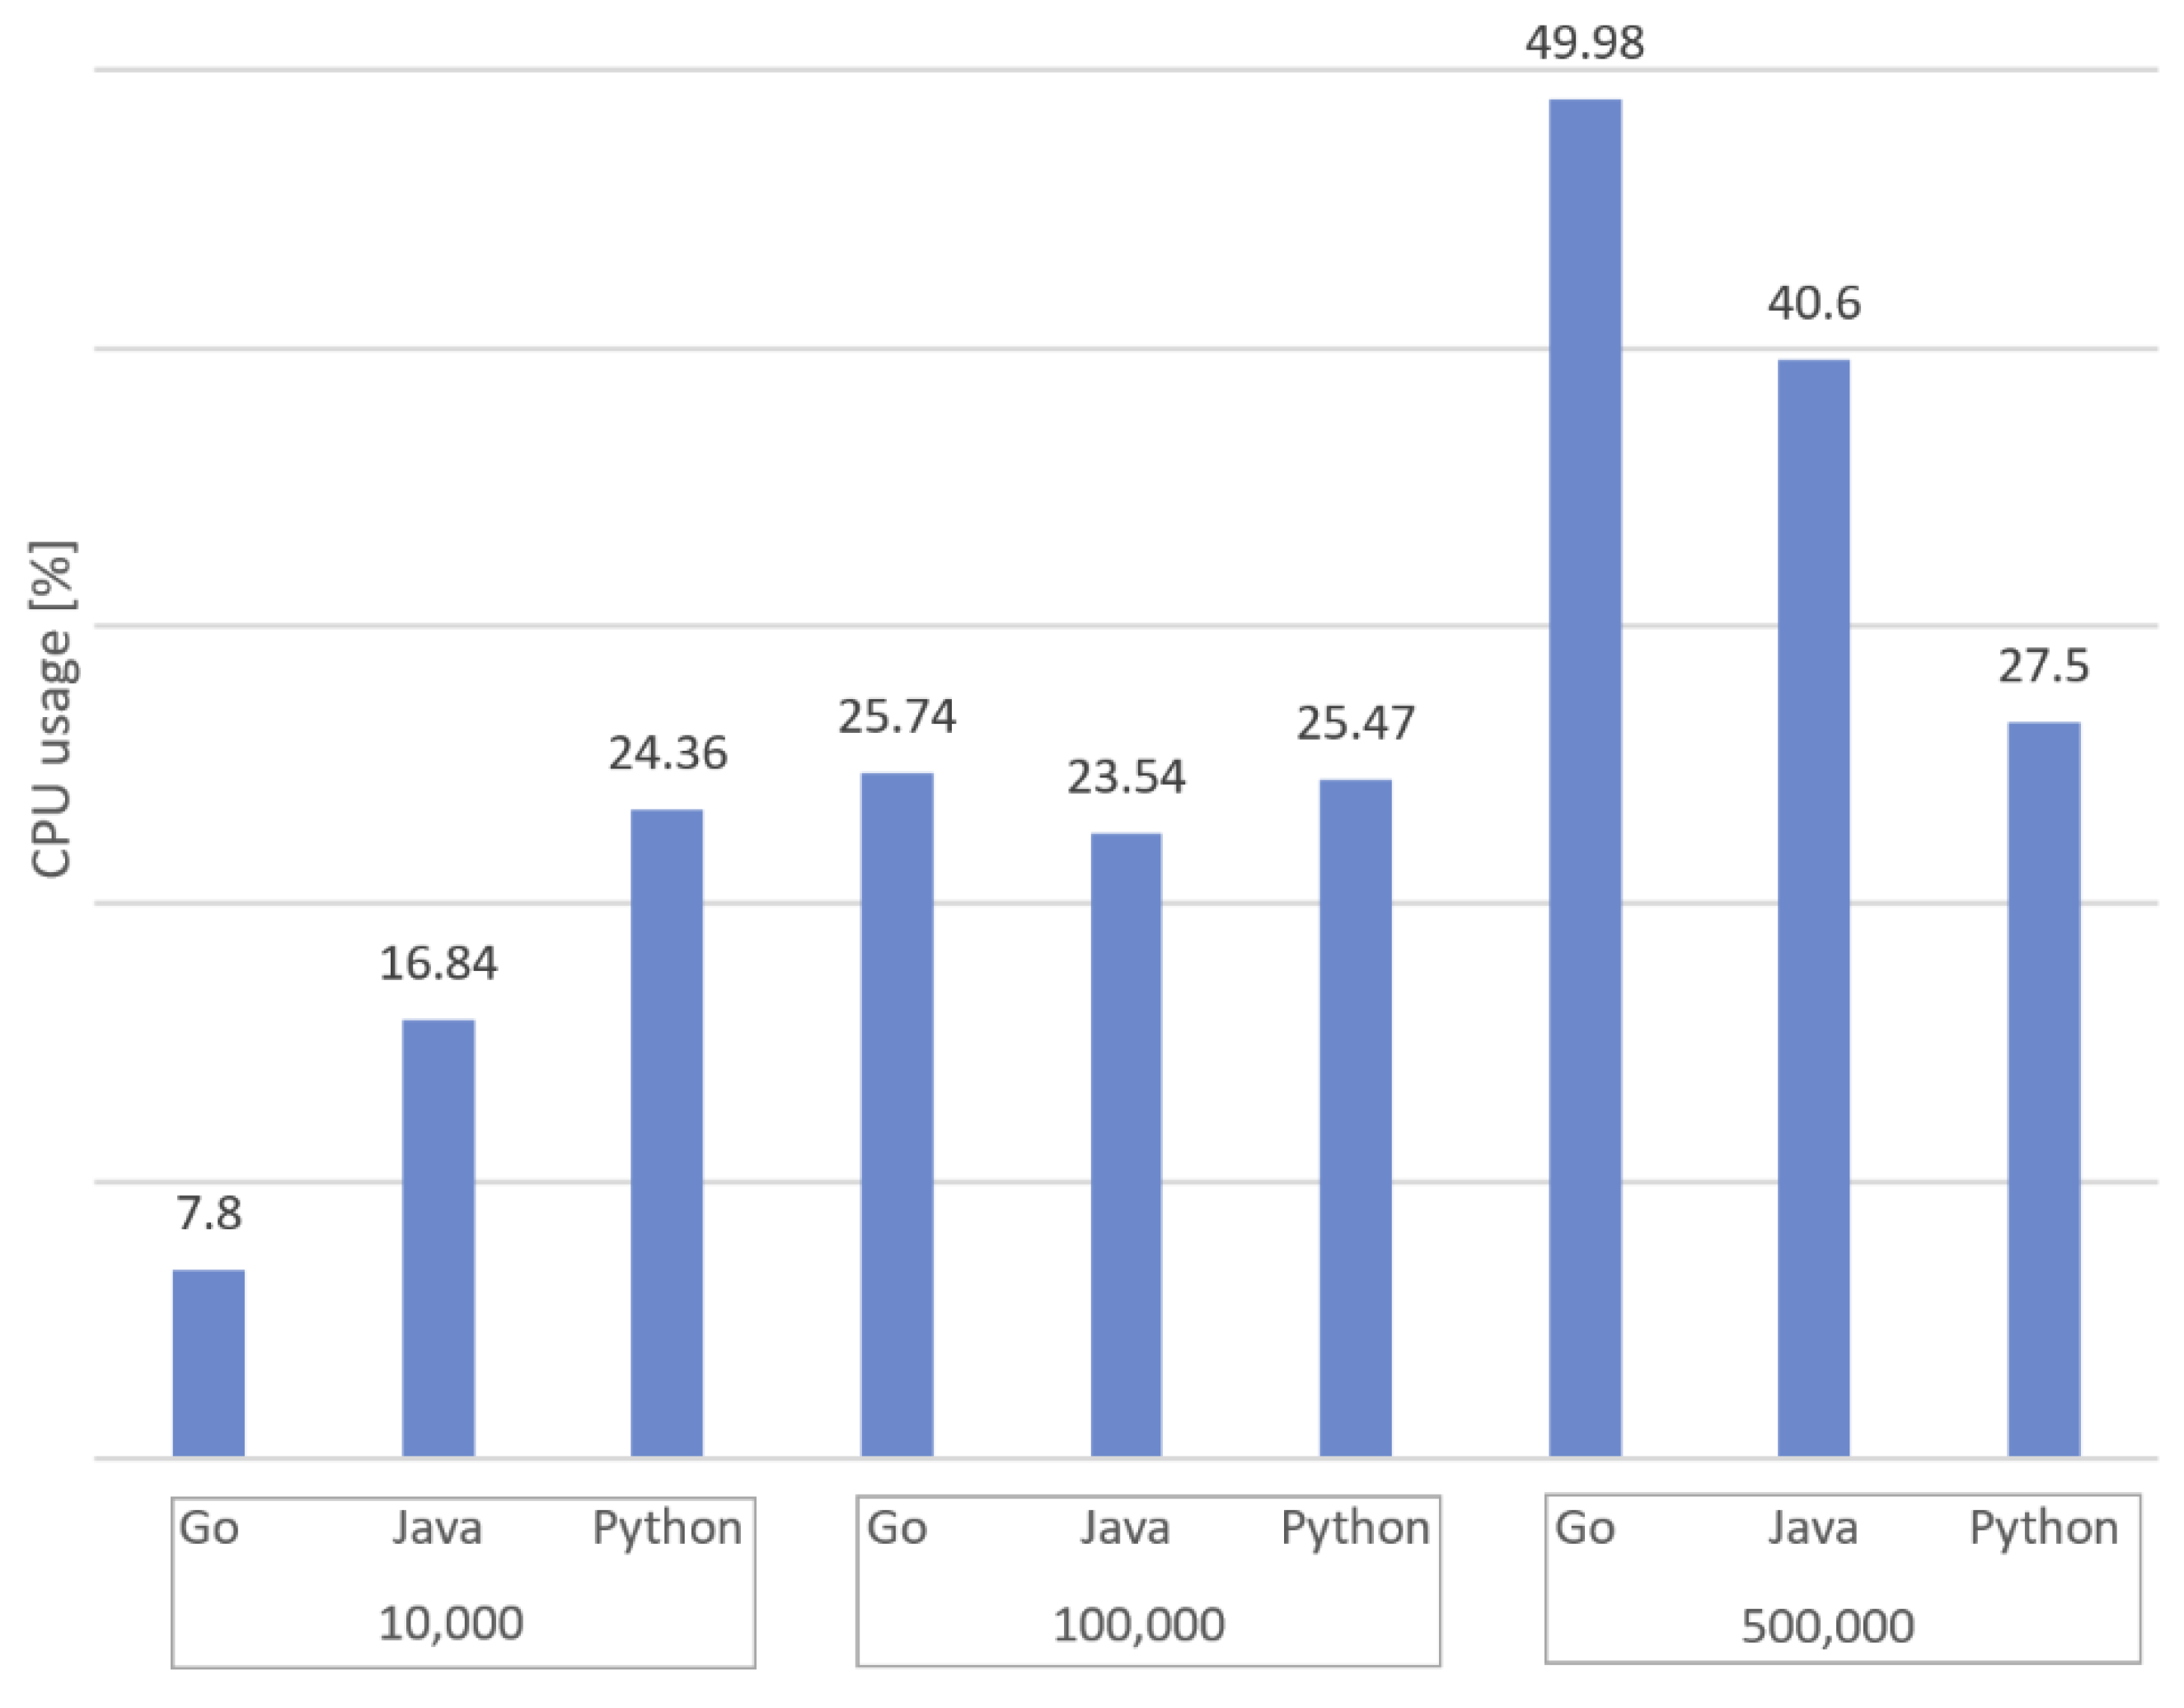
\includegraphics[height=0.3\textheight]{./part/Proyecto_ejecutivo/memoria_constructiva/golang/img/cpuUsage}
	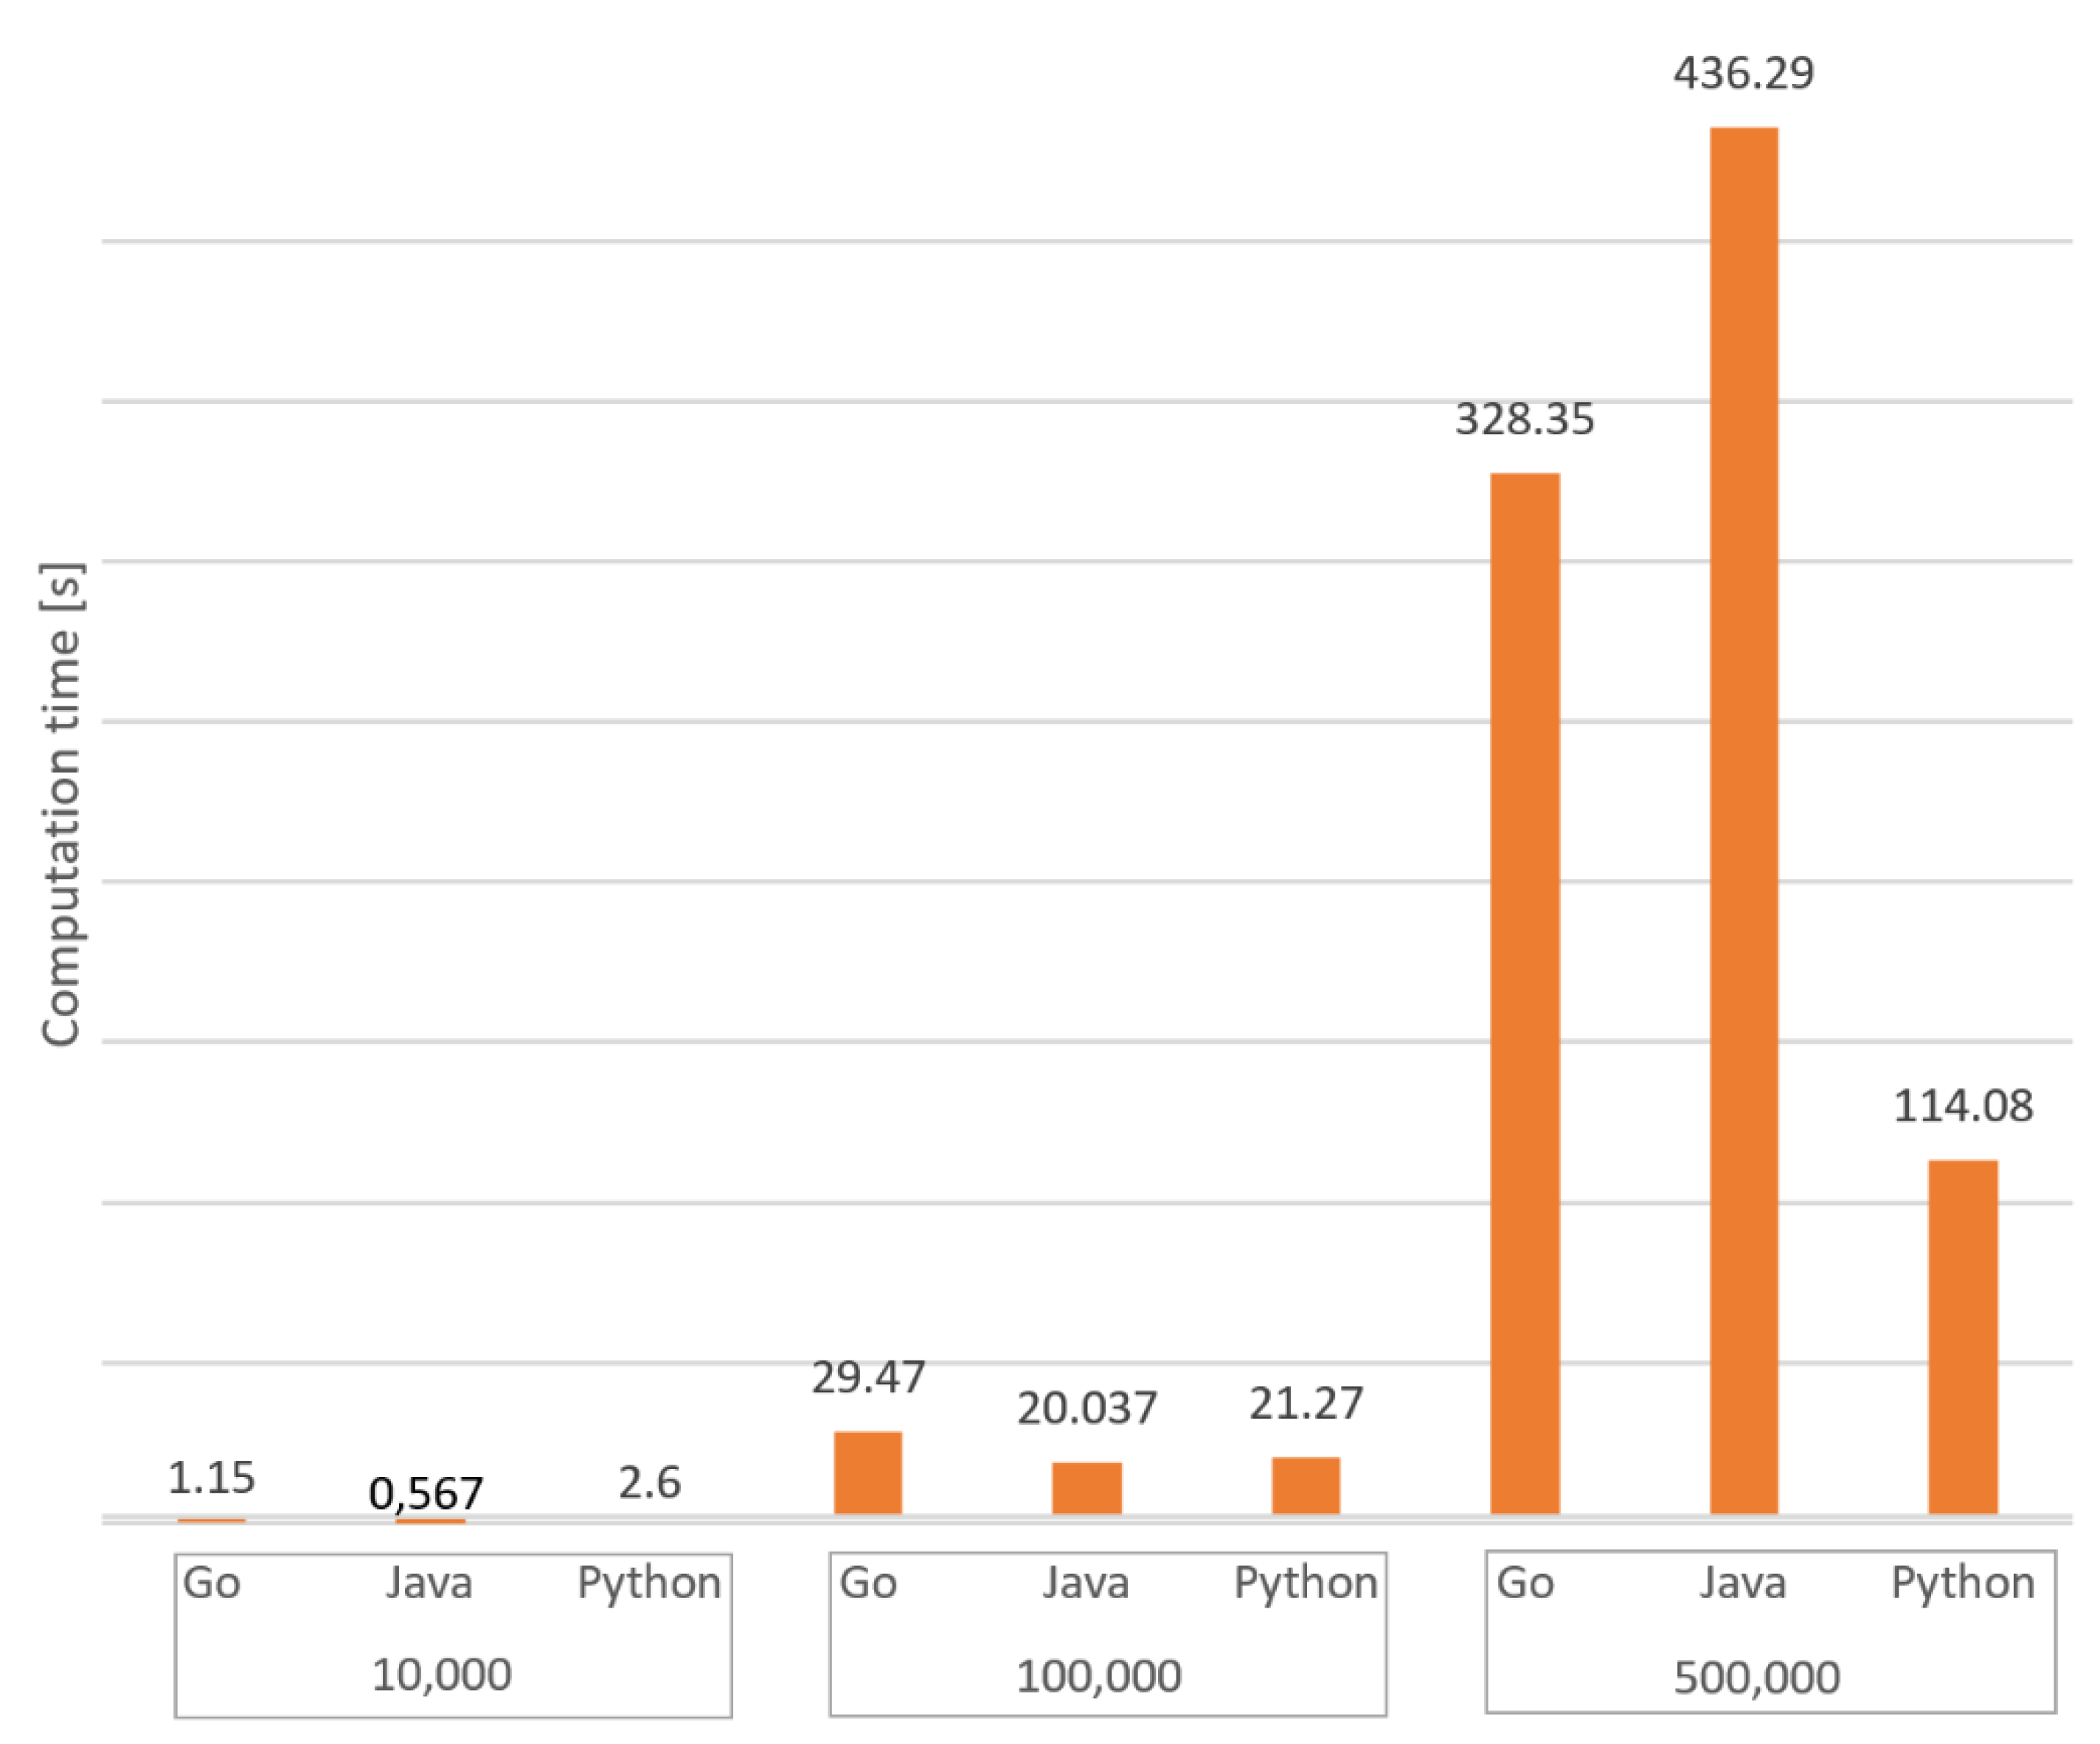
\includegraphics[height=0.3\textheight]{./part/Proyecto_ejecutivo/memoria_constructiva/golang/img/compTime}
	\caption[performance golang on algorithm]{performance golang on algorithm\cite{Dymora20201}}\label{fig:performance golang}
\end{figure}

El verdadero motivo para optar por golang como lenguaje para un software viene más de la mano de la facilidad de mantenimiendo, la rapidez de compilacion, el manejo fácil para la concurrencia y eficiente en el uso de recursos. Implementar mecanismos de memoria compartida para procesos concurrente es donde golang si optimiza recursos. Uno de los trabajadores de google que ha contribuido al ecosistema de go nos dice "Everyone knows and thinks about Google in terms of scale of users and scale of servers, but one thing that's not talked about as often is the scale of engineering effort."~\cite{Meyerson2014104+101}

Esto quiere decir que en la mayoría de las compañías el mayor coste no es el de infraestructura, si no el de ingeniería. Es un tradeoff muy importante el reducir el numero de horas dedicadas a mantener y desarrollar software que el hecho de optimizar el uso de máquinas. Si encima nos encontramos con un problema que no requiere de uso intensivo en cuestión algorítmica o tiempo de respuesta encontramos lo mejor de los dos: tenemos la ventaja de reducir los recuros necesarios de infraestructura y los de ingeniería. Si se diera el caso de que el software se enfrenta con el tiempo a problemas de escala siempre nos quedará la opción de aumentar las prestaciones de las máquinas utilizadas pero no tener problemas de aumento de costes de ingeniería

Es en la implementación de algoritmos que sacan ventaja de la concurrencia donde golang puede sacar ventaja respecto a otros lenguages como java o python ~\cite{Jenkins201714}

Estas son las principales conclusiones extraidas de la lectura de las publicaciones consultadas.
\cite{Effendy20211955}
\cite{Dymora20201}
\cite{Meyerson2014104+101}
\cite{Ray202110857}
\cite{Jenkins201714}
\cite{Ding2021321}
\cite{Taheri2021138}
\cite{NoAuthor2021179}
\cite{Dilley2019377}
\cite{Qiu2018}
\cite{Shoumik20181}
\cite{Mladenovic2018}
\cite{Benedict2017437}
\cite{Irawan2017}
\cite{Samaniego2017116}
\cite{Khaitan20152909}
\cite{Leokhin2015656}
\cite{Komendantskaya2014121}
\cite{Mittal2014292}
\cite{WhiteheadII2011209}
Nos permiten concluir que está justificado el uso en nuestro objetivo de diseñar un sistema de las carácteristicas de este proyecto con Golang.

Concluyo mencionando \cite{WhiteheadII2011209}"Despite the relatively young age of the programming language, we believe that Go helps
to fill an interesting niche in the field of programming languages. The unique feature-set and
aims of the language make it worth investigation for systems-level concurrent programming." Habiendo madurado el lenguaje unos años desde la publicación de este artículo encontramos que sigue siendo interesante, está altamente valorado en la comunidad.


    \paragraph{Estudio justificativo del uso de RPC}
        
La interacción entre los distintos servicios que se desarrollan en este proyecto se realizarán mediante una API. Entre los dos paradígmas más utilizados a la hora de crear APIs se encuentran RPC y REST. Se va a escoger el estandar RPC por responder a los requisistos a los que nos enfrentamos.

\textbf{GRPC}

Según el paper original que describe el paradígma RPC ¨Remote procedure calls (RPC) appear to be a useful paradig m for providing communication across a
network between programs written in a high-level language.¨ \cite{Birrell198439}

RPC permite ejecutar una llamada a un servicio en un servidor remoto mediante formularios predefinidos, obteniendo respuestas con el mismo formato. El estilo del servidor que realiza la llamada, no se tiene en cuenta por diseño.

Google Remote Procedure Call \cite{grpc} - es un subtipo del diseño RPC. gRPC es una arquitectura global de alto rendimiento y de código abierto RPC que garantiza la flexibilidad y la velocidad de la arquitectura de microservicios. Las llamadas a funciones se utilizan gRPC para garantizar la interacción con el cliente en los microservicios creados con varios lenguajes de codificación.

Esta técnica implementa las peticiones de la API en RPC utilizando el estándar HTTP 2.0, pero ni el servidor ni el programador de la API tienen conocimiento de HTTP. Como resultado, la complicación disminuye porque no hay que preocuparse por cómo se traducen los principios de RPC a HTTP.

La llamada a procedimientos remotos de Google pretende acelerar la transferencia de datos entre microservicios. Para permitir la devolución y la llamada remotas, se basa en una estrategia que identifica un servicio, establece las metodologías y especifica las variables pertinentes.

Además, utiliza un IDL -lenguaje de descripción de interfaces- para especificar el paradigma de la API RPC, lo que simplifica la identificación de las funciones remotas. El IDL emplea por defecto Protocol Buffers para definir la interfaz del servicio y el formato de los mensajes de carga útil.

\textbf{REST}

REST - Representational State Transfer - es un paradigma cliente-servidor se comunican a través de mensajes codificados en formato JSON o XML o compatibles.

En su disertación original del año 2000, Roy T. Fielding define REST como un "It means that a server will respond with the representation of a resource (today, it will most often be an HTML, XML or JSON document) and that resource will contain hypermedia links that can be followed to make the state of the system change. Any such request will in turn receive the representation of a resource, and so on." \cite{FieldingRoyThomas2000Asat}

Los principios que lo describen son:

\begin{itemize}
    \item Arquitectura cliente-servidor. Hace hincapié en la separación de responsabilidades.
    \item Ausencia de estado. El estado se guarda y mantiene en el cliente y no en el servidor
    \item Habilitación y uso de la caché. Todas las solicitudes deben declarar si son o no cacheables,
    \item Interfaz unifome
    \item Sistema por capas. Tiene relación con la separación de responsabilidades
\end{itemize}

Cada componente que combina el sistema de microservicios puede mostrarse al usuario o al cliente como un recurso cuando la API REST se hace accesible públicamente. Este recurso puede consultarse mediante los comandos HTTP GET, POST, PUT y DELETE .

En una API RESTful, el usuario envía una consulta a una URL - Localizador Uniforme de Recursos, que provoca una respuesta con una carga útil en JSON, XML o cualquier formato de datos compatible. Esta carga útil representa el recurso que desea el usuario. Las peticiones comunes de los clientes incluyen

\begin{itemize}
    \item Un método HTTP que especifica lo que debe procesarse en el recurso
    \item La ruta del recurso
    \item La cabecera que contiene datos sobre la consulta
    \item Una carga útil de mensaje específica del cliente
\end{itemize}

El servidor de la API envía una cabecera de tipo de contenido que identifica el formato de entrega del mensaje empleado en el cuerpo de la respuesta junto con la carga útil de datos que entrega al usuario que realiza la consulta. También se incluye en el cuerpo de la respuesta un código de respuesta que informa al usuario del estado del resultado de la llamada a la API.

\textbf{HTTP 1.1 frente a HTTP 2}

El protocolo HTTP/2 para transmitir mensajes permite flujos multiplexados y una comunicación bidireccional. gRPC admite varios tipos de interacciones, incluyendo interacciones unarias, streaming de servidor, streaming de cliente y streaming bidireccional. En contraste, REST utiliza el modelo de petición-respuesta de HTTP 1.1, lo que puede causar problemas de latencia y no aprovechar completamente las ventajas de HTTP/2. En general, gRPC puede proporcionar una transmisión de datos más rápida y eficiente y una comunicación más flexible y bidireccional en comparación con REST. HTTP 1.1, que permite REST, utiliza un método de handshaking TCP para cada consulta. REST Por ello, las APIs suelen tener problemas de latencia, ya que el handshake lleva tiempo.

\textbf{La estructura de datos de la carga útil}

Si nos fijamos en la estructura de datos de la carga útil, utilizada en el intercambio que se produce en la comunicación, gRPC utiliza Protocol Buffers para serializar y deserializar datos, lo que permite una transmisión más rápida y eficiente de información. Este método es más ligero, ya que los mensajes son una estructura más comprimida. Están en formato binario, lo que hace que el procesamiento sea menos intensivo en CPU. En el intercambio de datos, serializa y deserializa la información de forma automática.

Por otro lado, en REST, se utiliza principalmente JSON o XML para enviar y recibir información. La facilidad de lectura humana de JSON es una ventaja de REST, pero no es tan rápido o ligero cuando se trata de la transferencia de datos. Esto se debe al requerimiento de que JSON debe ser serializado y traducido a los lenguajes de programación utilizados en ambos extremos, el servidor y el cliente. Este paso adicional en el proceso de transmisión de datos puede afectar la eficiencia y aumentar la probabilidad de errores.


\textbf{Compatibilidad con los navegadores}

Dado que la mayor parte de la interacción de la API web se produce en línea, la compatibilidad con el navegador es una consideración clave en el debate entre gRPC vs. REST. La compatibilidad con los navegadores es probablemente una de las principales ventajas de las APIs REST frente a gRPC. Todos los navegadores ofrecen la capacidad completa de la API REST y la compatibilidad con el navegador. Sin embargo, para gRPC los navegadores sigue siendo relativamente restringida.

Para la comunicación entre HTTP 1.1 y HTTP 2 que necesita la interacción entre la web y gRPC se hace necesario establecer una capa proxy; lo cual presenta un elemento más de complejidad y mantenimiento, es por lo tanto un inconveniente en el uso de gRPC.

\textbf{Generación de código}

Para gRPC existe un compilador llamado protoc que carga los archivos .proto y genera código nativo para comunicarse con los servicios remotos que admite múltiples lenguajes de programación. En REST los ingenieros deben emplear herramientas de terceros, como Postman, para la generación de código para las consultas de la API.

La generación de código es especialmente ventajosa para los microservicios que combinan numerosos servicios creados en múltiples plataformas y lenguajes, facilitando la construcción del kit de desarrollo de software (SDK) para cada lenguaje y actualizándose de forma sencilla cuando se enfrenta a cambios.

\textbf{Justificación de uso de gRPC}

Aunque actualmente la mayoría de las herramientas de terceros no ofrecen una funcionalidad integrada para gRPC, es una tecnología adecuada para la interacción entre sistemas internos, como microservicios. Además, gRPC permite la interoperabilidad entre distintos lenguajes de programación, lo cual es otro de sus puntos fuertes. Esto se logra mediante el sistema generador de código, que se produce utilizando los archivos proto como interfaz de comunicación, lo que brinda una herramienta útil para aquellos que desean agregar funcionalidades mediante otro lenguaje y comunicarse fácilmente con el sistema ya existente. Todo lo que se necesita hacer es compilar los archivos proto en el lenguaje destino.

Otro beneficio del uso de gRPC es la transmisión de información en tiempo real mediante buffers de comunicación. En nuestro caso, el control en tiempo real de dispositivos mediante sistemas PID hace que esta característica sea esencial. gRPC permite establecer conexiones tanto de streaming por parte del cliente como del servidor, lo que nos permite establecer canales de comunicación versátiles según la situación a la que nos enfrentemos. Además, para la monitorización de los dispositivos controlados, necesitamos una optimización en el uso del ancho de banda. Aquí es donde gRPC sobresale, ya que proporciona una comunicación ligera, mayor eficiencia y rapidez.


Como resumén final hacemos referencia a a figura \ref{fig:gRPC vs REST} que resume la comparación entre los dos sistemas

\begin{figure}[H]
    \centering
    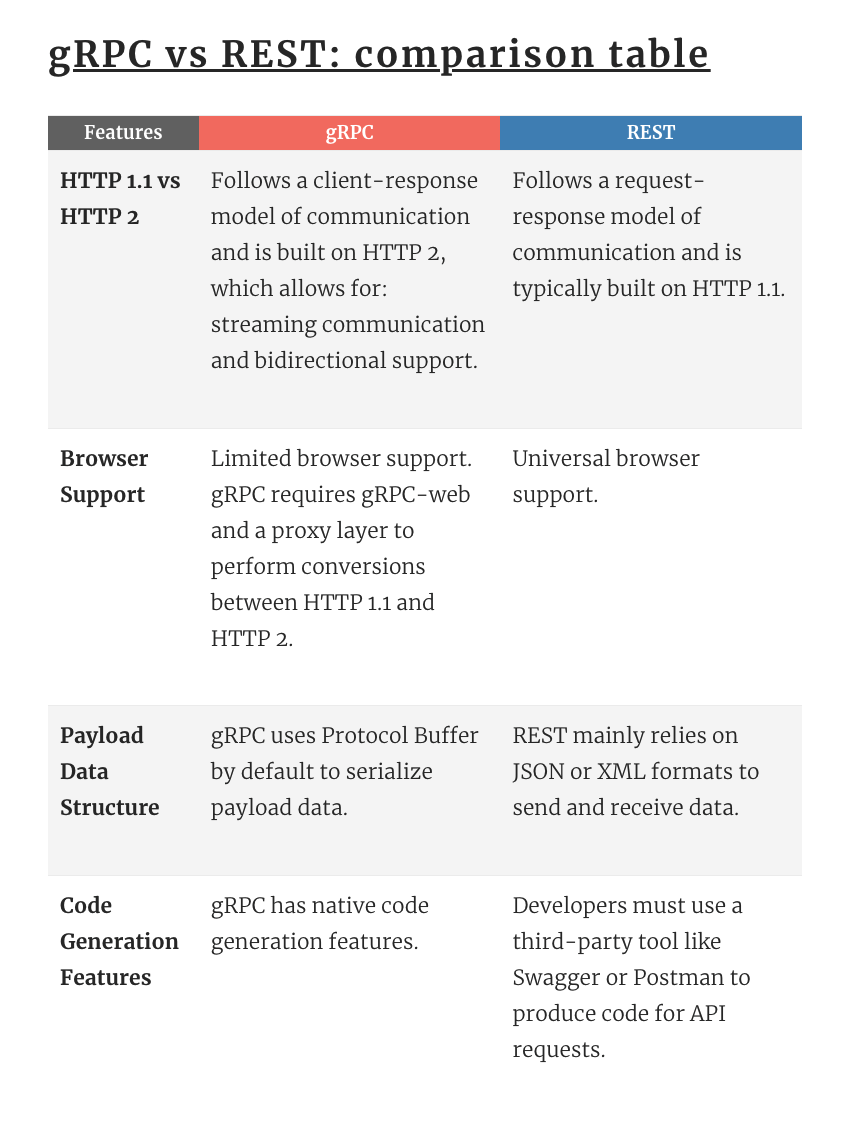
\includegraphics[height=0.3\textheight]{./part/Proyecto_ejecutivo/memoria_constructiva/rpc/img/rpcComparison}
    \caption{gRPC vs REST.\cite{berga_santos_2023}}\label{fig:gRPC vs REST}
\end{figure}
\subsubsection{Infraestructura}\label{subsubsec:infraestructura}
    \paragraph{Docker}\label{par:Docker}
        El fichero de definición de una imagen Docker se nombra por defecto como \textit{Dockerfile}.
Expresa la imagen base desde la que se parte, el fichero diseñado usa un sistema operativo debian, y se procede a ejecutar los distintos pasos de instalación de dependencias que se requieren para construir el contenedor.
En un mismo fichero Dockerfile existen distintos stages.
Un stage es cada conjunto de pasos diferenciados por un nombre.
A la hora de levantar el contenedor se puede seleccionar el requerido.
Esto es útil para, en un mismo fichero, especificar si queremos instalar las dependencias para desarrollo o producción.
Así se especifican y ahorran los elementos comunes, que de otro modo habrían de duplicarse y mantener en ficheros separados.
Los stages diseñados son: base, dev, compile y prod.

En la base se instalan los elementos comunes.
Si se especifica dev entonces se instala Golang, el debugger Delve, un usuario para evitar el uso de sudo dentro dicho container y distintas utilidades generales como git, vim como editor de textos y fish como terminal.
Si se construye mediante la etiqueta \textit{compile} se evita la instalación de los elementos de desarrollo y sólo instalamos golang para poder compilar el código.
En prod se usa esa fase primero para compilar.
Luego se parte de la base en limpio y se crea un contenedor con el ejecutable en su interior.
Ahorrando espacio en el contenedor.
Estos pasos pueden apreciarse en la~\cref{lst:dockerfile}.

La infraestructura consta además de una red para hacer visible los contenedores entre si: Manager, clients, base de datos y el proxy para el RPC\@.
La estructura se especifica en un archivo docker-compose.yml .~\cref{lst:dockercompose}.
Habrá un docker-compose.yml aparte para el proxy y la base de datos~\cref{lst:dockercomposegen}.

\phantom{blank}
\vspace{10mm}

\hrule

\begin{lstlisting}[language=docker-compose-2,caption={Docker-compose.yml para cada proyecto golang: Manager, client y control},breaklines=true,label={lst:dockercompose}]
version: "3.9"
services:
    web:
        container_name: go-manager
        build:
            context: .
            dockerfile: docker/Dockerfile
            target: $target
            args:
                GO_VERSION: 19.2
        image: go-manager:19.2-${target}
        ports:
            - "8081:8081"
            - "40000:40000"
        security_opt:
            - "seccomp:unconfined"
        cap_add:
            - SYS_PTRACE
        volumes:
            - .:/app
        tty: true

networks:
    default:
        name: pfm-network
        external: true
\end{lstlisting}


\hrule

\begin{lstlisting}[language=docker-compose-2,caption={Docker-compose.yml de sistemas compartidos y network},breaklines=true,label={lst:dockercomposegen}]
version: "3.9"

services:
  envoy:
    build:
      context: .
      dockerfile: ./envoy/Dockerfile
    image: grpcweb/envoy
    ports:
      - "8080:8080"
      - "9901:9901"
  mysql:
    image: mysql:8.0
    ports:
      - "127.0.0.1:3306:3306"
    container_name: mysql
    command: --default-authentication-plugin=mysql_native_password --general-log=1 --general-log-file=/tmp/mysql.log
    user: "1000:1000"
    environment:
      - MYSQL_ROOT_PASSWORD=$MYSQL_ROOT_PASSWORD
      - MYSQL_DATABASE=$MYSQL_DATABASE
    volumes:
      - pfm-db-data:/var/lib/mysql
volumes:
  pfm-db-data:
networks:
  default:
    name: pfm-network
    external: true
\end{lstlisting}


\hrule

\begin{lstlisting}[language=docker,caption={Dockerfile.yml},breaklines=true,label={lst:dockerfile}]
FROM debian:buster AS base

ARG GO_VERSION
RUN apt update && apt install -y curl

FROM base AS dev

WORKDIR /tmp

RUN apt update && apt install -y build-essential curl vim fish git sudo \
    && groupadd -g 1000 docker-user \
    && useradd -d /home/docker-user -s /bin/bash -u 1000 -g 1000 docker-user \
    && usermod -aG sudo docker-user && echo "docker-user:1234" | sudo chpasswd \
    && mkdir /home/docker-user \
    && chown -R docker-user:docker-user /home/docker-user

USER docker-user
WORKDIR /home/docker-user

RUN URL=https://storage.googleapis.com/golang/go1.${GO_VERSION}.linux-amd64.tar.gz \
        && curl ${URL} -o go.tar.gz  \
        && tar -zxf go.tar.gz  \
        && rm -rf go.tar.gz

ENV GOPATH /home/docker-user/go
ENV PATH $PATH:/home/docker-user/go/bin
ENV CGO_ENABLED 0

RUN go install github.com/go-delve/delve/cmd/dlv@latest
RUN ls -s /home/docker-user/go/bin/dlv /usr/local/bin

WORKDIR /app

FROM base AS compile

WORKDIR /tmp
RUN URL=https://storage.googleapis.com/golang/go1.${GO_VERSION}.linux-amd64.tar.gz \
        && curl ${URL} -o go.tar.gz  \
        && tar -zxf go.tar.gz  \
        && rm -rf go.tar.gz  \
        && mv go /usr/local/go

ENV GOPATH /usr/local/go
ENV PATH $PATH:/usr/local/go/bin
# If you enable this, then gcc is needed to debug your app
ENV CGO_ENABLED 0

WORKDIR /app
COPY ./app .
RUN go build -ldflags "-s -w" -o final.sh

FROM debian:buster AS prod

WORKDIR /
COPY --from=compile /app/final.sh /
CMD ["./final.sh"]
\end{lstlisting}

\hrule
    \paragraph{Raspberry}
        Necesitaremos una plataforma donde desplegar el programa de control que disponga de las características necesarias para interactuar con el hardware del  motor de corriente continua y la electrónica de potencia: el puente H. Las soluciones más comerciales son arduino y raspberry. Vamos a poner a prueba además la versatilidad de Golang para compilar el programa para distintas arquitecturas de forma trasparente para el programador. Facilitando su uso con distintas arquitectuas de chip.

Nos decantamos por raspberry por ser una interfaz más amigable de cara al desarrollo y las pruebas del programa. Se entiende que el ámbito del proyecto ya es lo suficientemente complejo y arduino pudiera requerir mayor de esfuerzo debído a no disponer de sistema operativo a la hora de trabajar.

\begin{figure}[H]
    \centering
    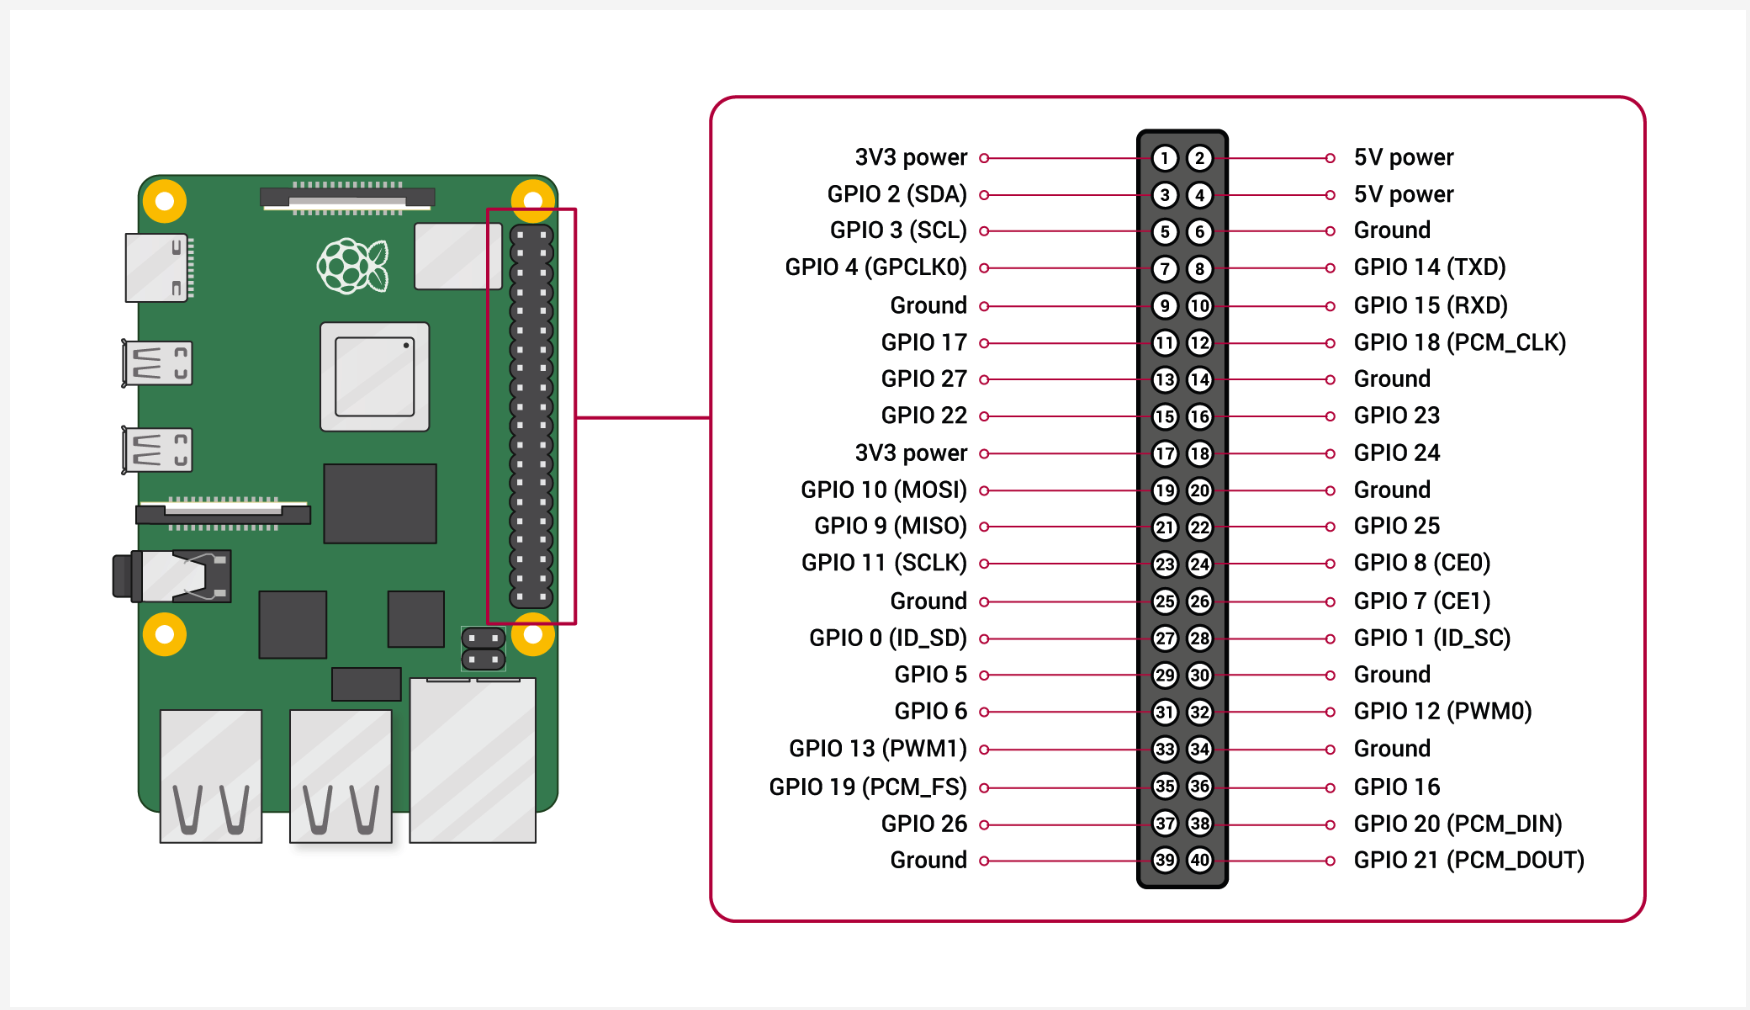
\includegraphics[scale = 0.4]{part/Proyecto_ejecutivo/memoria_constructiva/raspb/img/raspberry}
    \caption[Rasberry schema]{Raspberry schema \\Fuente: }\label{fig:raspberry pins}
\end{figure}

\begin{figure}[H]
    \centering
    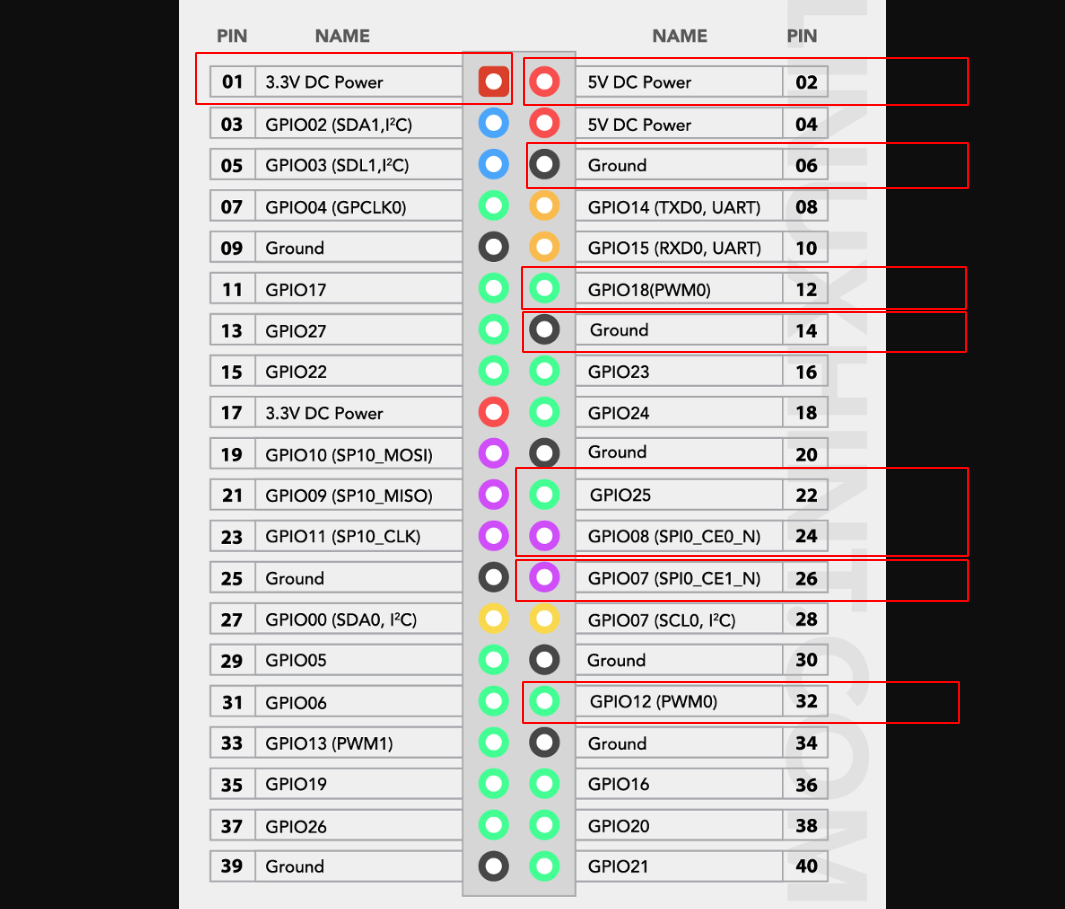
\includegraphics[scale = 0.4]{part/Proyecto_ejecutivo/memoria_constructiva/raspb/img/gpio-pinout-raspberry-pi-01-used}
    \caption[Motor EMG30]{Motor EMG30 \\Fuente: Documento de especificaciones técnicas.}\label{fig:Used Pins}
\end{figure}
    \paragraph{Motor CC y puente H}
        
El motor seleccionado será el~\cite{EMG30datasheet} Por el conocimiento que se dispone de su uso. En la figura~\cref{fig:EMG Motor} podemos apreciar su aspecto. Para el objeto que nos ocupa cumple con los requerimientos de ser sencillo, barato y disponer de una calidad suficiente.

\begin{figure}[H]
    \centering
    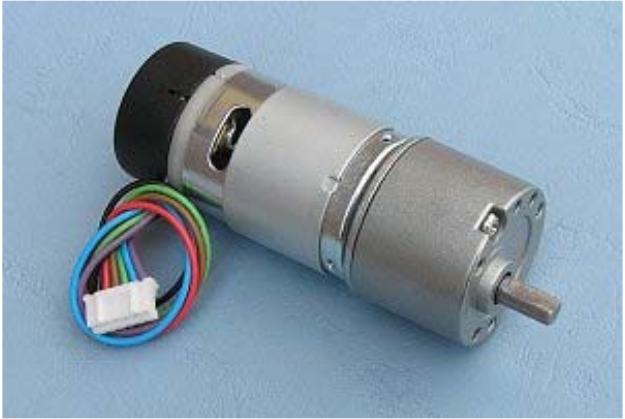
\includegraphics[scale = 0.4]{part/Proyecto_ejecutivo/memoria_constructiva/motor/img/MotorEMG30}
    \caption{Motor EMG30\cite{EMG30datasheet}}\label{fig:EMG Motor}
\end{figure}

Los parámetros que definen sus características más relevantes pueden apreciarse en la Tabla~\ref{tab:EMG30specifications}. El código de colores de las conexiones de las que dispone el motor podemos encontralo en las especificaciones ténicas del mismo. Se extraen en la~\cref{fig:motor connection}


\begin{table}[H]
    \centering
    \begin{tabular}{|l|l|}
        \hline
        Característica & Valor\\
        \hline
        Voltaje nominal & 12 V\\
        \hline
        Torque nominal & 1.5 kg/cm\\
        \hline
        Velocidad nominal & 170 rpm\\
        \hline
        Intensidad nominal & 530 mA\\
        \hline
        Velocidad sin carga& 216 rpm\\
        \hline
        Intensidad sin carga& 150mA\\
        \hline
        Intensidad máxima& 2.5 A\\
        \hline
        Salidad nominal & 4.22 W\\
        \hline
        Pasos por vuelta del codificador& 360 \\
        \hline
        Razón de la reductora & 30:1\\
        \hline
    \end{tabular}
    \caption{Características EMG30 \\ Fuente:\cite{EMG30datasheet}}\label{tab:EMG30specifications}
\end{table}


\begin{figure}[H]
    \centering
    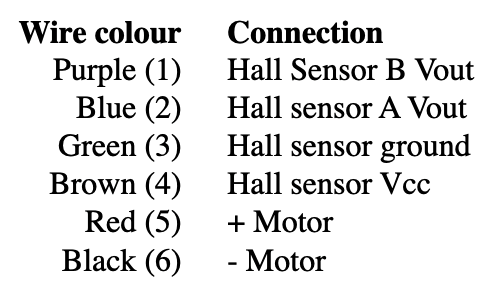
\includegraphics[scale = 0.6]{part/Proyecto_ejecutivo/memoria_constructiva/motor/img/motorConnection}
    \caption{Motor EMG30 \\Fuente: Documento de especificaciones técnicas.\cite{EMG30datasheet}}\label{fig:motor connection}
\end{figure}


        El componente utilizado para ampliar la señal enviada por el Arduino al motor, sirviendo de intermediario entre éste y los motores es el módulo específico para el control mediante PWM de motores con un circuito integrado LMD18200T que soporta hasta tres Amperios. En definitiva es un puente H controlado por PWM.\\

Ha sido elegido por satisfacer todas los requisitos necesarios en nuestra tarea: Precio, voltaje, amperaje y de implementación sencilla. Este módulo podría fabricarse, dado su sencillez, a mano comprando los componentes por separado, sin demasiado esfuerzo.\\
\begin{figure}[H]
		\centering
		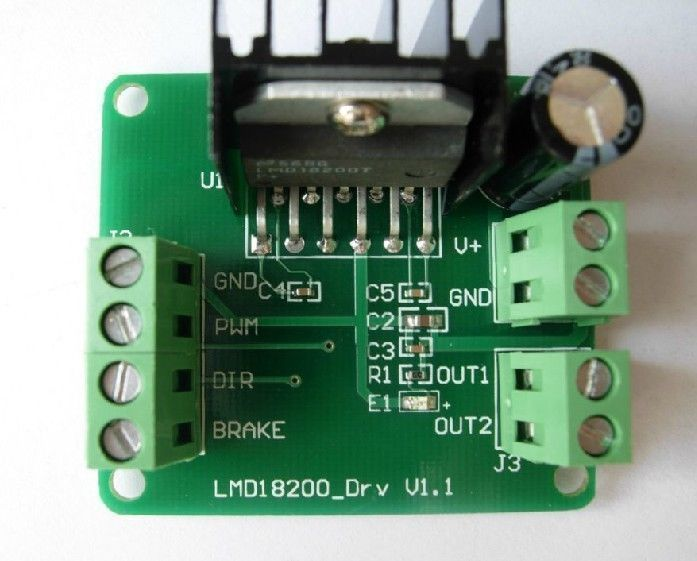
\includegraphics[scale = 0.3]{part/Proyecto_ejecutivo/memoria_constructiva/motor/img/modulopot}
		\caption[Módulo de potencia.]{Módulo de potencia.\\Fuente: \url{http://i.ebayimg.com/}(2014)}\label{fig:figure}
\end{figure}
	
Se aprecian en la figura 6 las entradas y las salidas de las que dispone. De arriba abajo la primera columna es de entradas:

\begin{itemize}
	\item \textbf{GND:} La tierra de la placa de control, en nuestro caso el Arduino.
	\item \textbf{PWM(Pulse width modulation):} la señal del control por ancho de pulsos.
	\item \textbf{Dir:} Señal con el sentido de giro que se desea.
	\item \textbf{Brake:} Freno del motor
\end{itemize}

Y la segunda columna de alimentación y salidas:

\begin{itemize}
	\item \textbf{V+:} Alimentación de 12 voltios.
	\item \textbf{GND:} tierra.
	\item \textbf{OUT1:} Salida de una mitad del puente H.
	\item \textbf{OUT2:} Salida de la otra mitad del puente H
\end{itemize}

La composición del circuito conocido como puente H y su implementación en este módulo viene detallada en el ANEXO donde se referencia al manual del circuito integrado.

		\textbf{Conexión}
El esquema de conexión hacia los elementos con los que interactúa es el siguiente:
\begin{figure}[H]
		\centering
		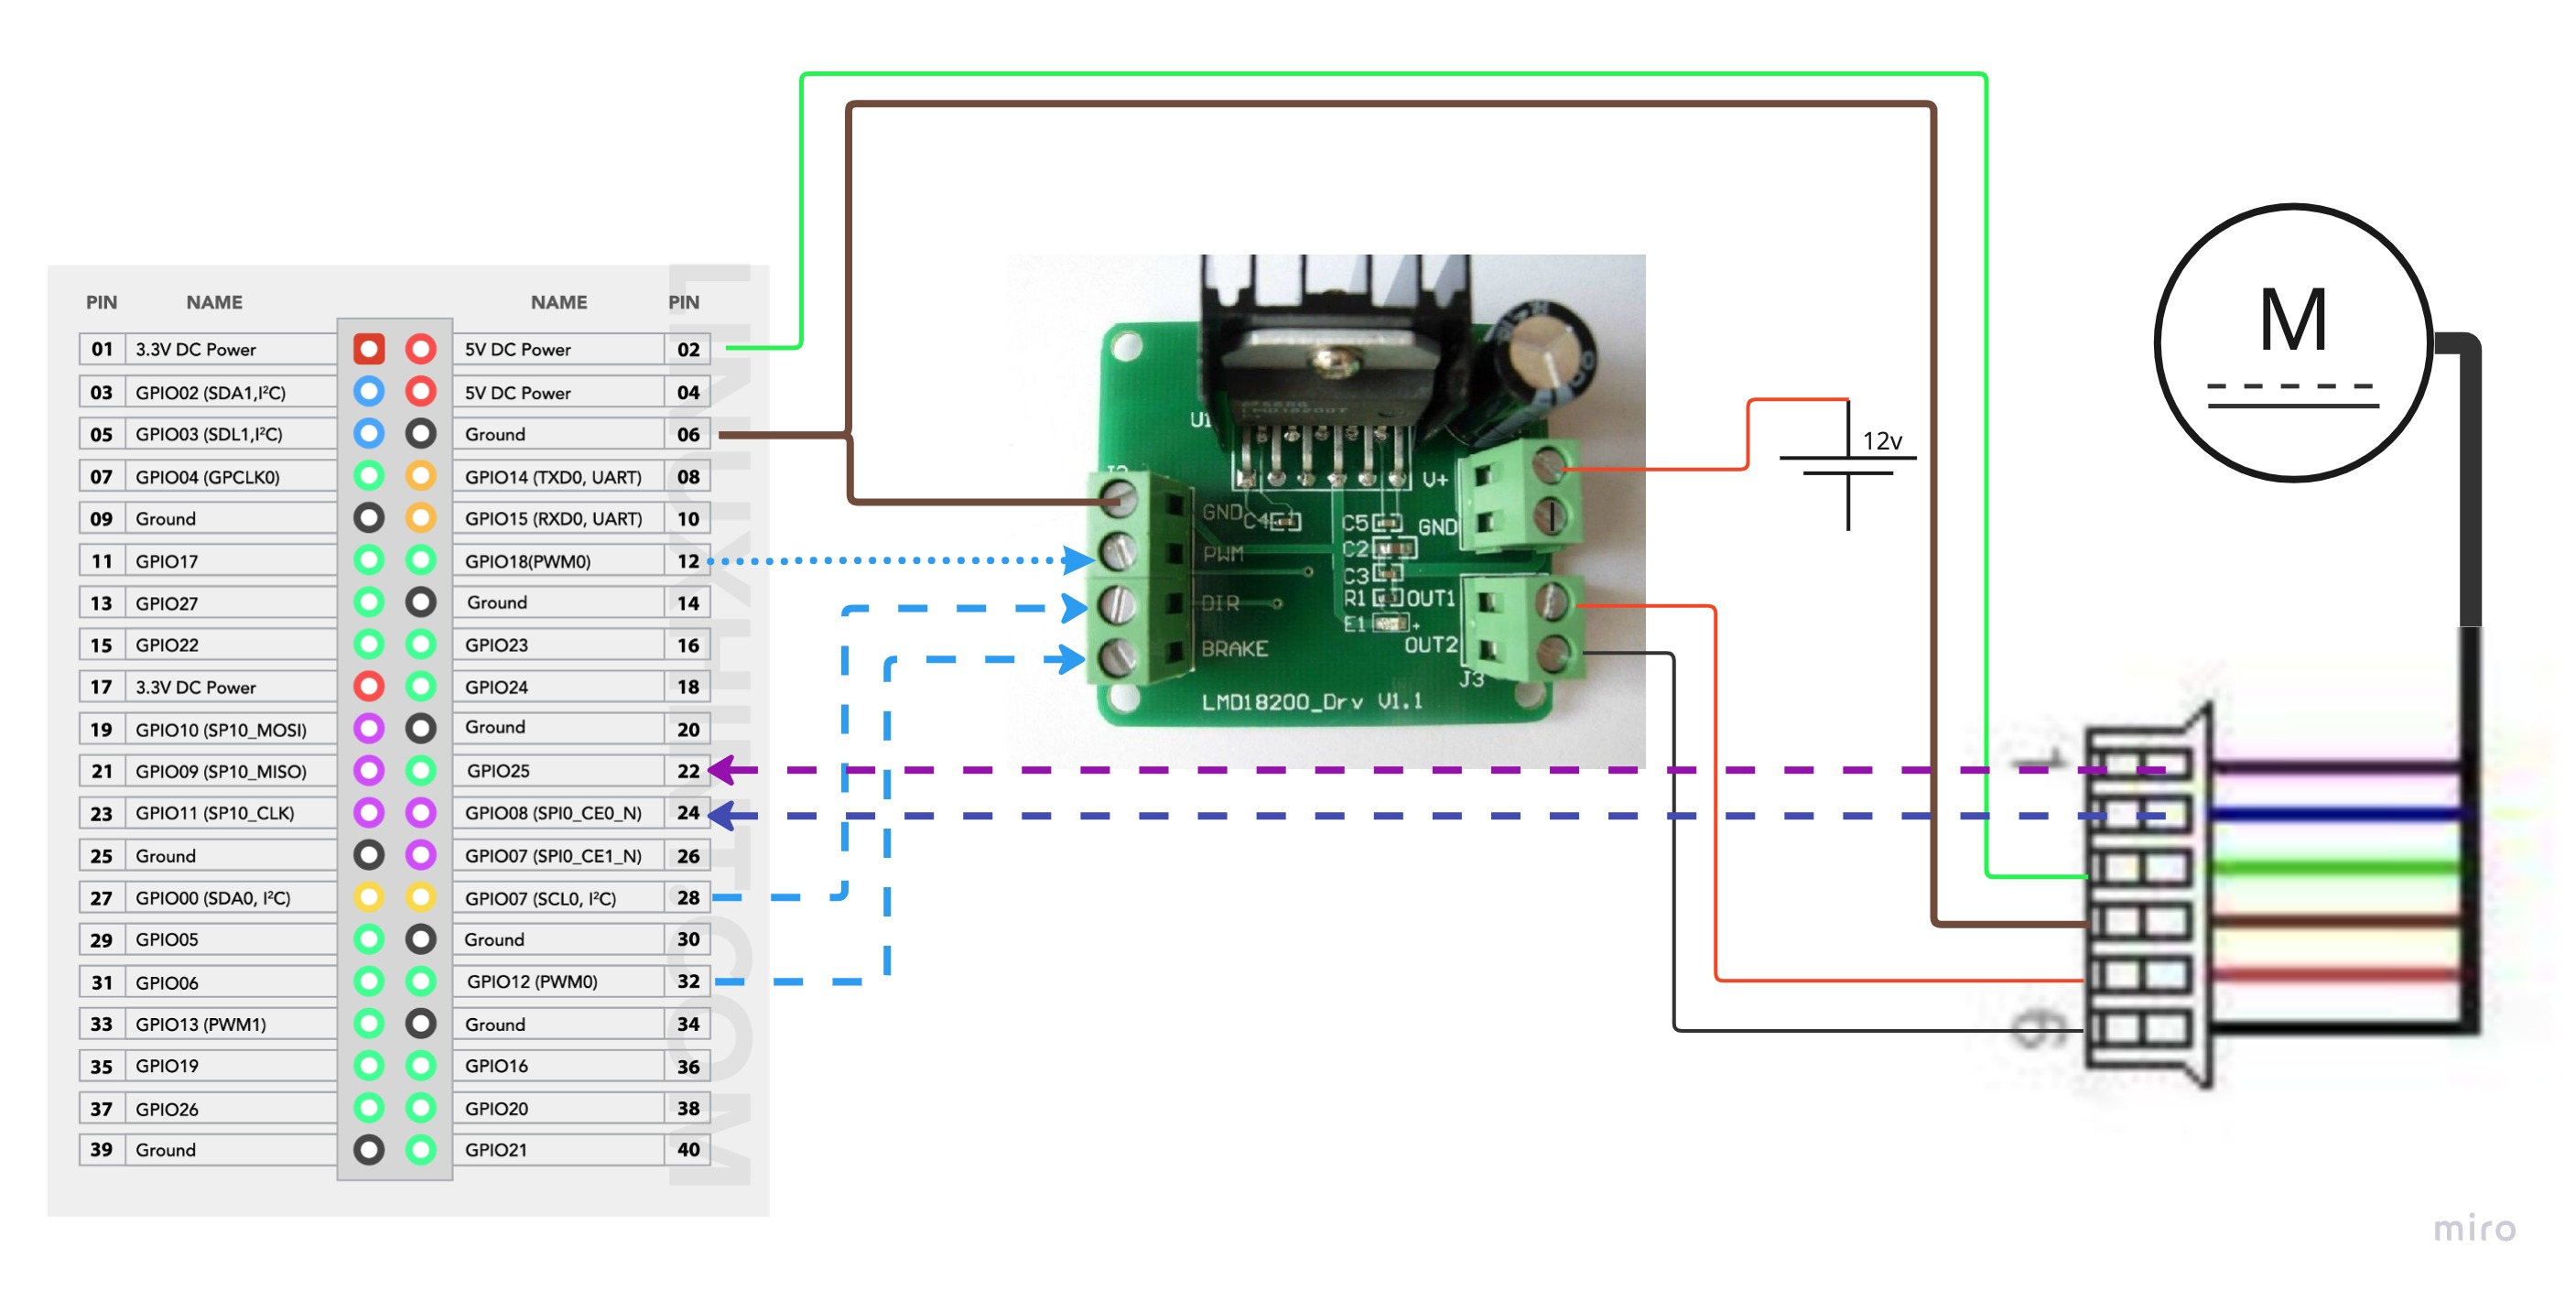
\includegraphics[scale = 0.15]{part/Proyecto_ejecutivo/memoria_constructiva/motor/img/connection diagram}
		\caption[Esquema de conexión del módulo de potencia.]{Esquema de conexión del módulo de potencia.\\Fuente: elaboración propia.}\label{fig:figure2}
\end{figure}
    \paragraph{Mysql}\label{par:mysql}
        Para la base de datos escogeremos Mysql por ser también la solución más estandar.
        Al tener conocimiento previos de su uso evitamos añadir mayor esfuerzo de investigación.
        Podemos ver en la figura~\cref{fig:DBSchema} El digrama de relaciones entre los distingos elementos de la base de datos.
        Esta base de datos permitirá persistir la información introducida por los usuarios en el sistema del programa Manager.\\

        \begin{figure}[H]
            \centering
            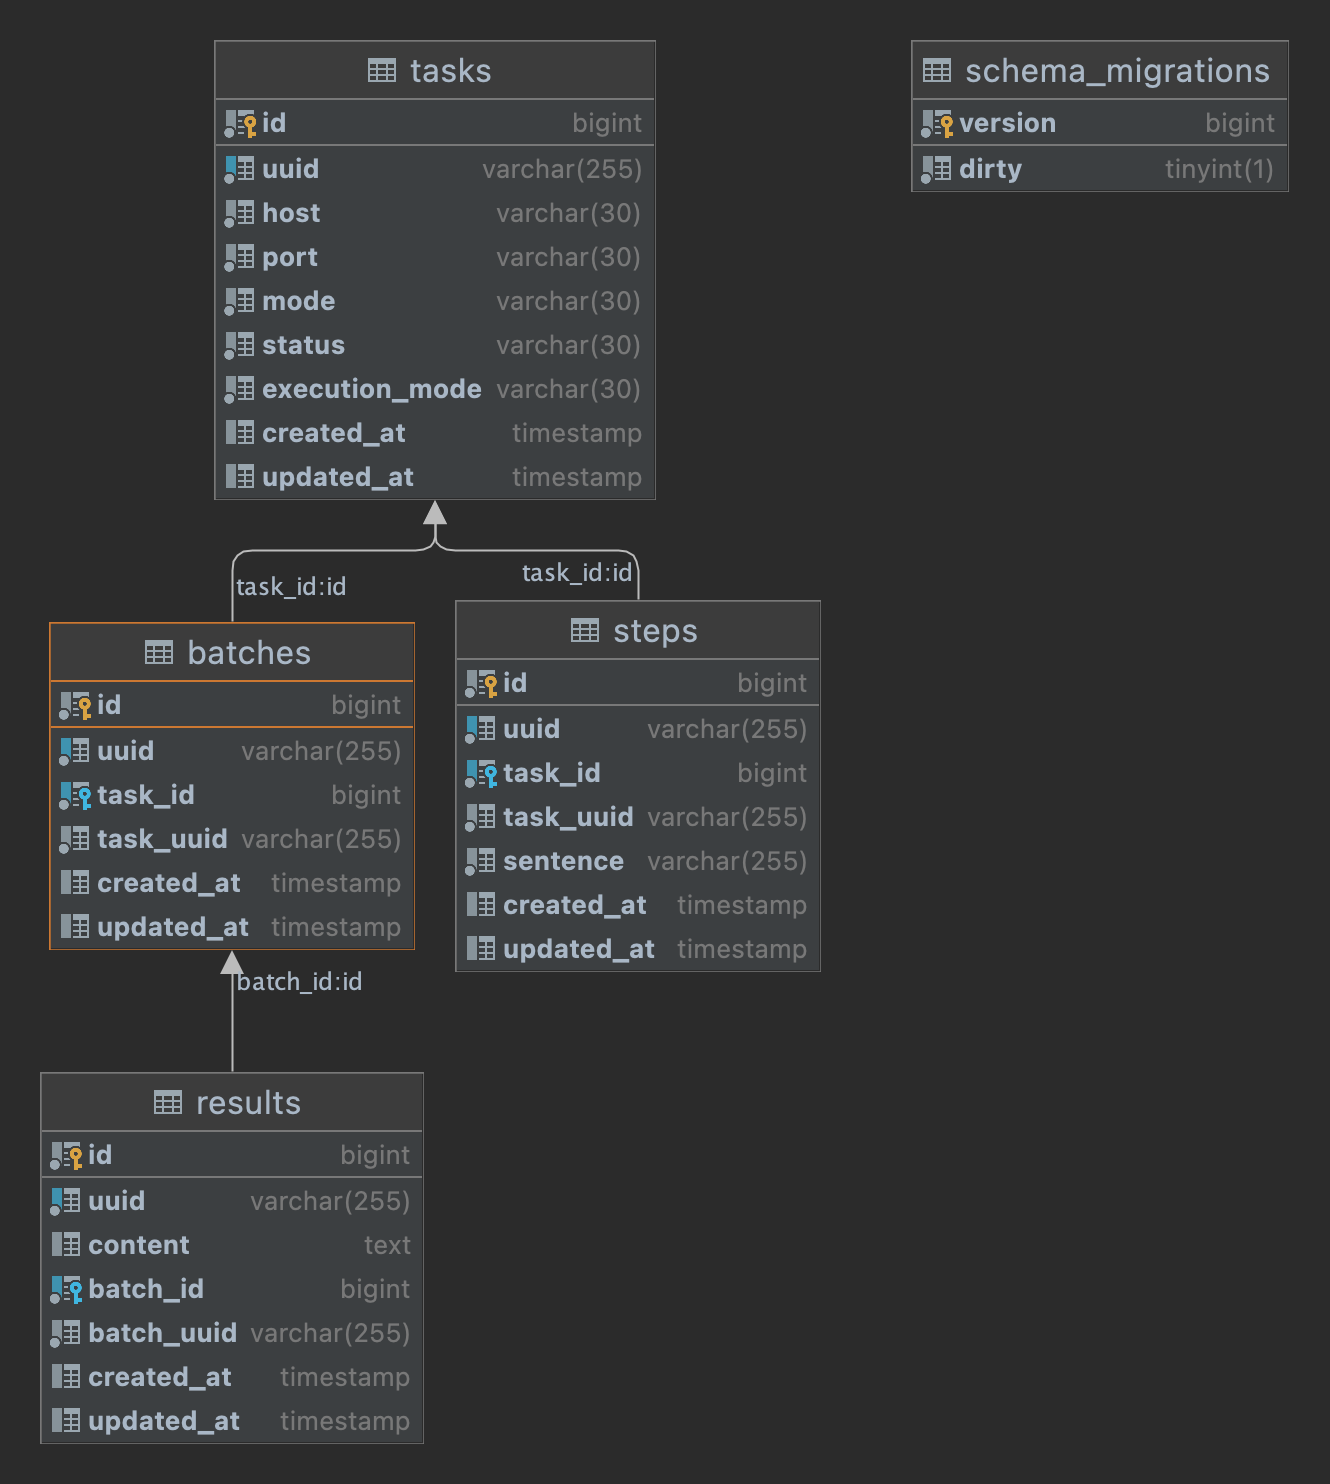
\includegraphics[scale = 0.2]{part/Proyecto_ejecutivo/memoria_constructiva/dbSchema}
            \caption{Esquema de la base de datos}\label{fig:DBSchema}
        \end{figure}
    \paragraph{CI/CD}\label{par:cicd}
        Para garantizar la correcta entrega del software cada vez que se añada código a la versión en produccion se ejecutarán scripts automáticos.
        El programa más extendido para el control de versiones de software es Git y el servicio de almacenamiento en la nube de control de versiones git más extendido es Github.
        Github pone a nuestra disposición el servicio de Github Actions.
        Es un servicio automatizado que lanza los scripts configurados a lo largo del flujo de vida del código en el control de versiones.

        Podemos ver en la ~\cref{fig:cicd} configurado que se ejecuten nuestros scripts en los Pull Request y en el proceso final de unión de código nuevo a producción.
        Los Pull Request son el proceso anterior a introducir código nuevo en producción.
        Se realiza una petición de revisión a los colaboradores del repositorio antes de introducir dicho código.
        En el mismo proceso de revisión antes de que los compañeros acepten dicha contribución pueden ver que se han ejecutado los scripts que garantizan que dicho código pasa todos los tests y siguen el estándar de estilo.
        En el proceso de unión final se volverán a ejecutar los mismos.

        \begin{figure}[H]
            \centering
            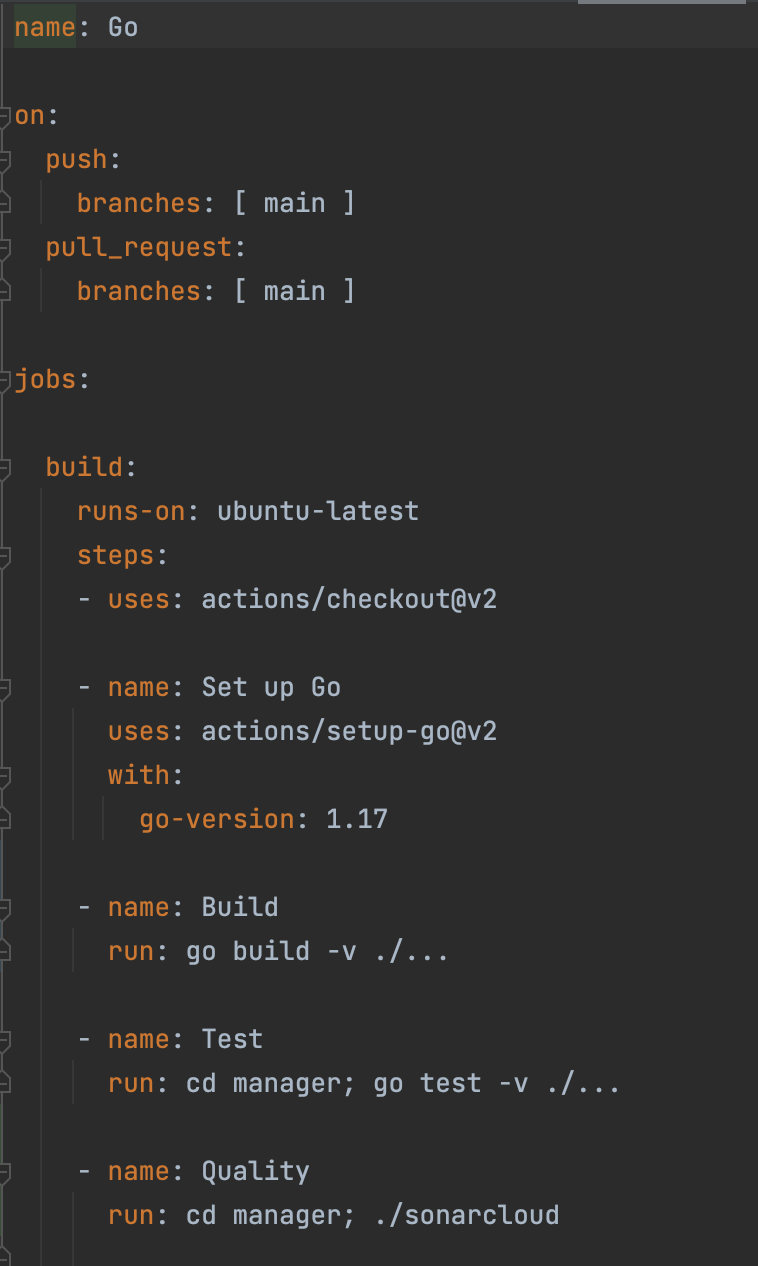
\includegraphics[scale = 0.7]{part/Proyecto_ejecutivo/memoria_constructiva/cicd}
            \caption{Github actions}\label{fig:cicd}
        \end{figure}